\subsection{Bestimmung der Wei�lichtpositon der polychromatischen Strahlung des Muffelofen}
Bei wei�em Licht gibt es nur an der Wei�lichtposition konstruktive Interferenz, da an dieser Positon der Gangunterschied gleich 0 ist. Die Wei�lichtposition des Muffelofen liegt also in Abh�ngigkeit der Spiegelpostion dort, wo die Intensit�t maximal wird. Neben der Wei�lichtposition kann von einer Gleichverteilung zwischen konstruktiver- und destruktiver Interferenz ausgegangen werden. Bei der Suche nach dem Wei�lichtpunkt wurden zwei Kandidaten gefunden. 

Der erste Wei�lichtpunkt wurde bei 4,7545(80) mm gefunden, siehe Abbildung \ref{fig:weisslichtpunkt_1}. Der zweite Wei�lichtpunkt wurde bei  5,770(3) mm gefunden, sieh Abbildung \ref{fig:weisslichtpunkt_2}. Die Herkunft des zweiten Wei�lichtpunktes ist nicht bekannt.

\begin{figure}[H]
\centering
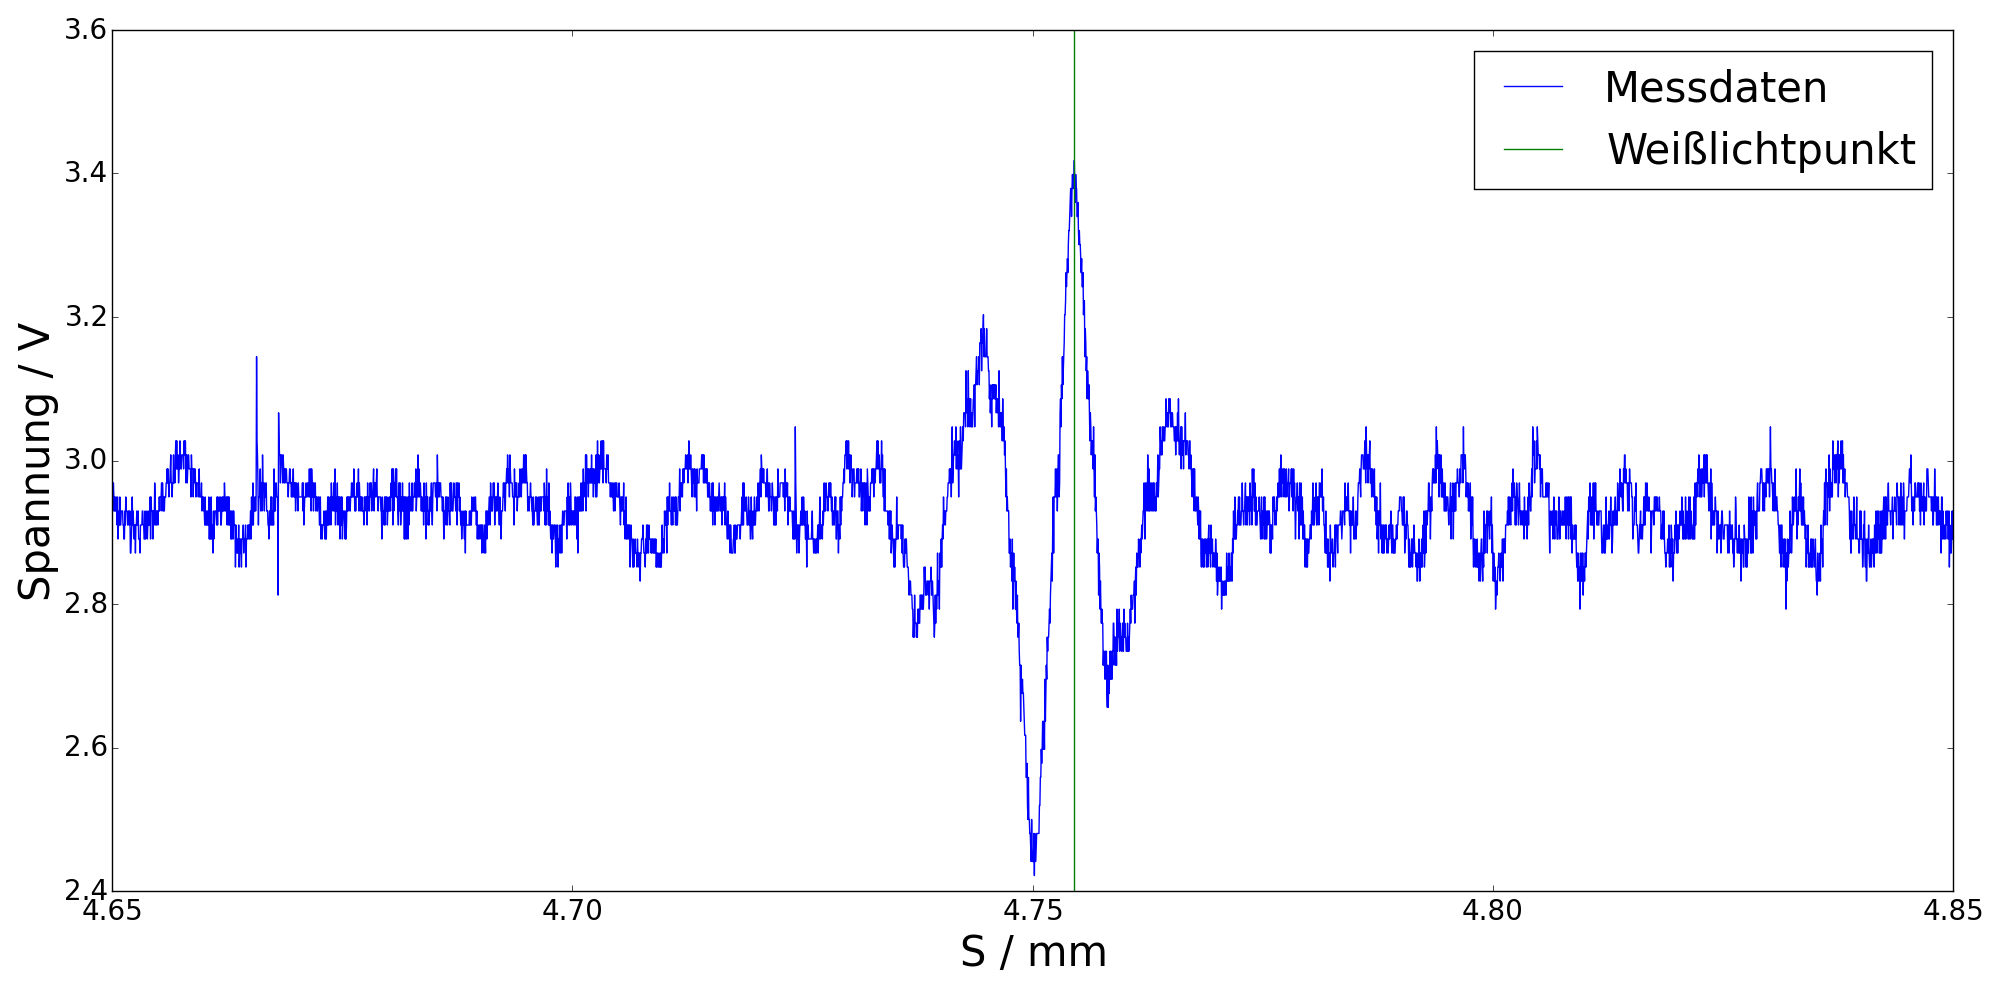
\includegraphics[scale = 0.33]{weisslichtpunkt_4,77.png}
\caption{Erster bestimmter Wei�punkt bei 4,755(8) mm}
\label{fig:weisslichtpunkt_1}
\end{figure}

\begin{figure}[H]
\centering
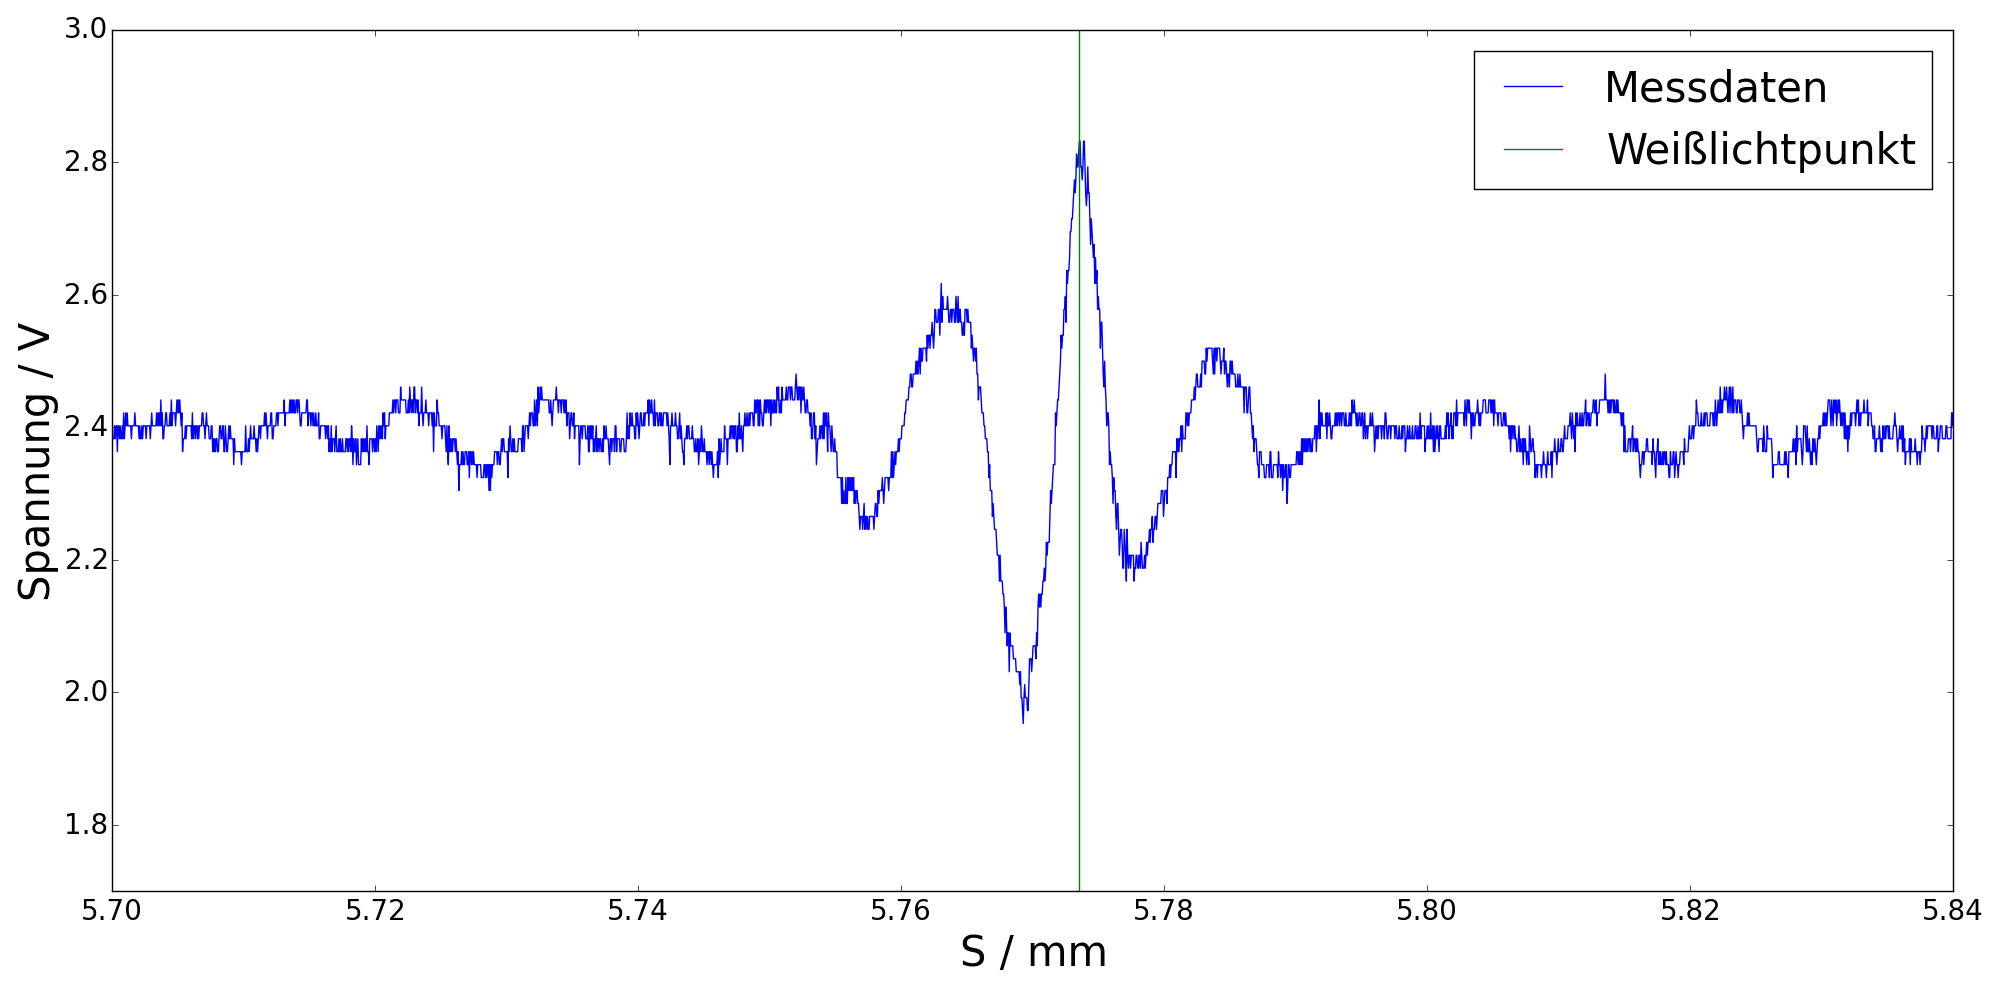
\includegraphics[scale = 0.33]{weisslichtpunkt_5,8.png}
\caption{Zweiter bestimmter Wei�punkt bei 5,770(3) mm}
\label{fig:weisslichtpunkt_2}
\end{figure}

Die beiden Plots, f�r die Eichung des Abstandes und die Tabellen mit den Parametern sind im Anhang in Abschnitt \ref{subsec:weisslicht} zu finden.